% Format papel A4 and fleqn (left align equations)
\documentclass[a4paper,fleqn]{cas-sc}


% type of cited references
%\usepackage[numbers]{natbib} 
\usepackage[authoryear]{natbib}
%\usepackage[authoryear,longnamesfirst]{natbib}

%%%Author macros
\def\tsc#1{\csdef{#1}{\textsc{\lowercase{#1}}\xspace}}
\tsc{WGM}
\tsc{QE}
%%%


\begin{document}
\let\WriteBookmarks\relax
\def\floatpagepagefraction{1}
\def\textpagefraction{.001}

% Short title
\shorttitle{Applied and Computational Harmonic Analysis}    
% Short author
\shortauthors{C. Paredes, G. Rosario, J Valero.}  

% Main title of the paper
\title [mode = title]{Money growth and inflation in China: New evidence from a wavelet analysis}  

% Title footnote mark
% eg: \tnotemark[1]
%\tnotemark[<tnote number>] 

% Title footnote 1.
% eg: \tnotetext[1]{Title footnote text}
%\tnotetext[<tnote number>]{<tnote text>} 


% First author
%
% Options: Use if required
\author[1]{Christian Paredes}
%[type=editor,
       %style=chinese,
       %auid=000,
       %bioid=1,
       %orcid=0000-0000-0000-0000,
       %facebook=<facebook id>,
       %twitter=<twitter id>,
       %linkedin=<linkedin id>,
%       gplus=<gplus id>]

% Footnote of the second author
%\fnmark[1]

% Address/affiliation
\affiliation[1]{organization={Department of applied mathematics, Universitat Polit\`ecnica de Val\`encia},
            addressline={Camino de Vera s/n}, 
            city={Val\`encia},
            postcode={46022}, 
            country={Spain}}

% Email id of the first author
\ead{clparagu@posgrado.upv.es}


% Second author
%
% Options: Use if required
\author[2]{Gabriel Rosario}%[<options>]

% Corresponding author indication
\cormark[1]

% Email id of the second author
\ead{garoro4@alumni.uv.es}

% Address/affiliation
\affiliation[2]{organization={Departament de Matem\`atiques, Universitat de Val\`encia},
            addressline={C/ Dr. Moliner, 50}, 
            city={Val\`encia},
            postcode={46100}, 
            country={Spain}}

% Corresponding author text
\cortext[1]{Corresponding author}

% For a title note without a number/mark
%\nonumnote{}

% Third author
\author[3]{Jorge Valero Mira}%[<options>]
\ead{garoro4@alumni.uv.es}
\affiliation[3]{organization={Department of mathematics, Universidad de Alicante},
            addressline={San Vicente del Raspeig}, 
            city={Alicante},
            postcode={03690}, 
            country={Spain}}

% Here goes the abstract
\begin{abstract}
    This paper provides a fresh new insight into the dynamic relationship between money growth and inflation in China by applying a novel wavelet analysis. From a time-domain view, our findings show strong but not homogenous links between money growth and inflation in the mid-1990s and the period since the early 2000s. Especially since the early 2000s, China\'s monetary policy has achieved much better performance in terms of inflation management compared to previous years. From a frequency-domain view, we find that money growth and inflation are positively related in one-to-one fashion in the medium or long run whereas they deviates from such a positive relation in the short run due to temporary shocks and significant lag effects. We can also conclude for China that the long-run relationship between $M_0$ growth and inflation supports the modern quantity theory of money (QTM), while the medium-run relationship between $M_1$ growth and inflation as well as $M_2$ growth and inflation supports the modern QTM. In general, however, our results fit well with the fact that China has experienced economic transitions and structural adjustments in monetary policy over the past two decades. Based on the above analysis, this paper provides an overall view of monetary policy operations and some beneficial implications for China.
\end{abstract}

% Keywords
% Each keyword is seperated by \sep
\begin{keywords}
    \sep Money growth
    \sep Inflation
    \sep Wavelet analysis
    \sep Time domain
    \sep Frequency domain 
\end{keywords}

\maketitle

% Main text
\section{Introduction}
China has experienced striking money growth over the past several decades. Statistics from China's central bank, the People's Bank of China (PBoC), show that China's broad money (M$_2$) reached up to $118.2$ trillion Yuan by the end of May 2014. This means that China's M$_2$ has increased by four times over the last 10 years, with an average year-on-year growth rate of $40.3\%$ during the past decade. On a global scale, China's M$_2$ has also been $1.7$ times as much as that in the U.S. and even $1.5$ times as much as that in the Euro area.\footnote{Statistics from the U.S. Federal Reserve Bank and the Euro Central Bank show that the stock of M$_2$ reached $11.23$ trillion dollars in the U.S. and $12.73$ trillion dollars in the Euro area by the end of May 2014.} Moreover, the ratio of M$_2$ to gross domestic product (GDP) is as high as $194.5\%$ in China at the end of 2013. However, the ratio is just $97.9\%$ in the Euro area and $65.8\%$ in the U.S.,\footnote{Statistics from the U.S. Bureau of Labor Statistics, the Eurostat and the National bureau of statistics of China show that at the end of 2013, the GDP for China is about $9.3$ trillion dollars whereas it is $16.8$ trillion dollars for the US and $12.9$ trillion dollars for the Euro area.} although the two economies have implemented several rounds of Quantitative Easing (QE) in the aftermath of the global financial crisis. As a consequence, many are concerned with such striking money growth coupled with such a high ratio of M$_2$ to GDP would bring substantial inflationary pressures to the Chinese economy. In addition, a long-run unity relationship between money growth and inflation established by the quantity theory of money (QTM) increases this concern. If the QTM holds true in China, then high money growth would ultimately threaten future price stability and hence the economic growth. Therefore, we are greatly motivated to re-assess the relationship between money growth and inflation in China by using a novel method and the most recent data and with special attention paid to whether such a relationship in China supports the QTM. In addition, as we well know, the money supply has been the intermediate target of monetary policy, while inflation management has been the ultimate target since the mid-1990s in China. As a result, the relationship between money growth and inflation can reflect the effectiveness of monetary policy implementation to a large degree. In this sense, it is worthwhile to explore such a relationship to shed light on what has happened to China's monetary policy over the past several decades.

This paper proposes a novel wavelet analysis to revisit the relationship between money growth and inflation in China. Wavelet analysis is greatly distinctive from most conventional mathematical methods such as time-domain methods (correlation analysis and Granger causality, etc.), which cannot identify short-run and long-run relationships between time series, and frequency-domain methods (Fourier analysis, etc.), which cannot reveal how such relationships change over time. It allows us to expand time series into a time-frequency space in which the local correlation and the lead-lag relationship can be read off in a highly intuitive way. Therefore, it is very suitable for assessing simultaneously whether the relationship varies across frequencies and evolves over time. In addition, a wavelet analysis has a significant advantage over the well-known Fourier analysis, especially when the time series under study are non-stationary or locally stationary \cite{ROUEFF2011813}.

Wavelet analysis was introduced into economics by \cite{Goffe1994}, \cite{ramsey1998decomposition,ramseylampart1998} in the mid-1990s. However, its extensive applications in economics did not emerge until recent years. A strand of literature uses wavelet coherency and phase differences based on the continuous wavelet transform (CWT) to assess co-movements between stock markets as well as between energy commodities and macroeconomy (\cite{RUA2009}; \cite{grahanikkinen2011}; \cite{Aguiar-Conraria2011}; \cite{maccarthyOrlov2012}; \cite{VACHA2012}; etc.). Another strand of literature applies multi-resolution analysis based on the maximal overlap discrete wavelet transform (MODWT) to reexamine some of the most investigated relationships in empirical economics (\cite*{GALLEGATI2011}; \cite*{HACKER2014}; \cite{REBOREDO2014}). For example, \cite{GALLEGATI2011} test for the stability of the wage Phillips curve relationship across frequencies and over time. \cite{REBOREDO2014} provide new evidence of the effects of oil prices on stock returns for the U.S. and Europe. \cite{HACKER2014} revisit the causal relationship between spot exchange rates and nominal interest rate differentials. Wavelet studies that attempt to discuss problems regarding monetary policy and inflation have also been undertaken in recent years. \cite*{AGUIARCONRARIA2008} reveal the time-frequency effects of the U.S. monetary policy on its macroeconomy. \cite*{dowd2011} presents a wavelet-based method to estimate the U.S.'s core inflation. \cite*{AGUIAR2012} explore the time- and frequency-varying relationship between the yield curve shape and macroeconomy for the U.S. \cite{Rua2012} examines the dynamic relationship between money growth and inflation for the Euro area.\footnote{\cite{Rua2012} uses the same kind of methods to analyze a similar problem as the present paper does, but the employed data of these two papers come from different countries, and their focuses of attention are also largely different.} To date, no work has utilized wavelet analysis to examine the dynamic relationship between money growth and inflation in China, which is another large motivator for us to make an attempt.

This study differs from those in the existing literature in several important ways. First, wavelet analysis devotes special and full attention to the time-frequency relationship between money growth and inflation in China. Second, this paper employs the most recent monthly data of inflation and money growth, ranging from January 1991 to June 2014. Third, through estimating wavelet power spectrums, wavelet coherencies and phase differences among growth rates of M$_0$, M$_1$, and M$_2$ and inflation rates, respectively, we unravel the extent to which money growth and inflation comprehensively relate to each other, how such a relationship evolves with time, which rate is the leader and whether short-run and (or) long-run relations exist between them in China. Finally, our empirical results show high but not homogenous links between money growth and inflation over time and across frequencies that fit with the fact that China has experienced economic transitions and structural adjustments over the past two decades. In general, this paper provides additional and useful implications for China's monetary policy.

The rest of the paper proceeds as follows. \hyperref[sec:2]{Section 2} briefly reviews the literature on the relationship between money growth and inflation. \hyperref[sec:3]{Section 3} provides an overview of wavelet theory and methods. \hyperref[sec:4]{Section 4} introduces data and plots wavelet power spectrums. \hyperref[sec:5]{Section 5} presents the empirical results and policy implications. \hyperref[sec:6]{Section 6} concludes.

\section{Related literature}\label{sec:2}
As mentioned above, it is well known that the relationship between money growth and inflation is historically associated with the QTM. The traditional QTM suggests a unitary relationship between money growth and inflation (\citealp{fisher1911}). However, the modern QTM argues that money growth impacts both output and inflation in the short run but would be completely reflected on inflation in the long run (\citealp{friedman1956}). Despite the remaining dispute about the short-run relationship, both the traditional and modern QTM, however, reach an agreement with the unitary relationship between money growth and inflation in the long run.

Entering the 1990s, a large number of empirical studies emerged to investigate the relationship between money growth and inflation for different countries. While some studies find a unidirectional or bidirectional causal relationship between money growth and inflation (\citealp*{ASSENMACHER2008}; \citealp*{HALL2009}; \citealp*{hossain2005}; \citealp*{liu2002}), additional studies that follow the research patterns of the QTM suggest a positive relationship between them from a shortrun and (or) long-run view. \cite{xie2004}, \cite{roffia2007}, \cite*{Zhang2012} and \cite*{Yu2012} claim that money growth has a positive impact on inflation in the short run, whereas \cite*{mccandless}, \cite{crowder1998}, \cite{christensen}, \cite{Grauwe2005}, and \cite{Zhang2008,zhang2009,Zhang2012,Yu2012} argue that money growth has a positive impact on inflation in the long run. \cite*{MacCandless1995} as well as \cite{Grauwe2005} reach almost the same conclusion that money growth and inflation are related one-for-one in the long run, which provides strong support for the QTM, particularly for modern QTM. There is also limited work that presents a negative relationship between money growth and inflation. For example, \cite{shuai2002} and \cite{wu2002} find that China's money growth has an unusually negative impact on inflation in the 1993–2001 period. 

For a further consideration, \cite{lucas1980} presents for the first time that the frequency level should not be ignored when examining the relationship between money growth and inflation. More recent work has paid special and extensive attention to how money growth and inflation relate at different frequencies (\citealp*{ASSENMACHER2008b,ASSENMACHER2008a}; \citealp*{benati2009}; \citealp*{bruggeman2005}; \citealp*{haug1880}). While some researchers focus on the frequency-varying relationship between money growth and inflation, there has been another strand of literature that examines whether such a relationship evolves over time (\citealp*{BASCO2009}; \citealp*{Christiano2003}; \citealp*{liu2012}; \citealp*{milas2009}; \citealp*{rolnick1997}; \citealp{sargent2008}; \citealp{zhang2009}. For example, \cite{zhang2009} demonstrates that inflation persistence in China has been significantly weakened since 1997 as a consequence of systematic improvements in monetary policy. \cite{liu2012} Liu find that their link has become weaker over the past decade in China.

Limited work performs a simultaneous assessment of how money growth and inflation relate at different frequencies and how such a relationship evolves over time, with the exception of \cite{Rua2012}, who achieves this using wavelet analysis. Using wavelet coherency and phase difference tools, he finds that the relationship between money growth and inflation is stronger at low frequencies and that money growth in the Euro area seemed to lose its leading properties with respect to inflation in the past decade. In this paper, we have also proposed to apply the wavelet analysis to investigate the dynamic relations between money growth and inflation in both the time and frequency domains. However, despite using a similar method, this paper employs the distinctive monthly data for China spanning from January 1991 to June 2014, which implies that we devote special attention to the world's biggest developing country to the effects of high money growth on inflation, and the ensuing findings would provide some additional and helpful implications for China's monetary policy implementation.

\section{Wavelet theory and methods}\label{sec:3}
Wavelet analysis originated in the mid-1980s as an alternative to the well-known Fourier analysis. Although Fourier analysis can uncover the relations across different frequencies by means of spectral techniques, the time-localized information is completely discarded under the Fourier transform. Moreover, Fourier analysis is only suitable for stationary time series. In contrast, wavelet analysis allows us to estimate the spectral characteristics of a time series as a function of time and then extracts localized information in both time and frequency domains (\citealp{AGUIARCONRARIA2008}). In addition, wavelet analysis has significant superiority over the Fourier analysis when the time series under study are non-stationary or locally stationary \cite{ROUEFF2011813}.

\subsection{The continuous wavelet transform}
As the beginning of the wavelet analysis, wavelet transform decomposes a time series into stretched and translated versions of a given “mother wavelet” that is well-localized in time and frequency domains. In this way, the series can be expanded into a time-frequency space where its time- and (or) frequency-varying oscillations are observed in a highly intuitive way. Often, two classes of wavelet transforms exist: discrete wavelet transforms (DWT) and continuous wavelet transforms (CWT). The DWT is useful for noise reduction and data compression, while the CWT is more helpful for feature extraction and data self-similarity detection (\citealp*{grinsted2004}; \citealp*{loh2013}). As such, the CWT is widely used in economics and finance (\citealp{AGUIARCONRARIA2008}; \citealp{caraiani2012}; \citealp{Rua2012}).

Given a time series $x(t)\in L^2(\mathbb{R})$, its CWT in regard to the mother wavelet $\psi(t)$ is defined as an inner product of $x(t)$ with the family $\psi_{\tau,s}(t)$ of "wavelet daughters"\footnote{Here, $L^2(\mathbb{R})$ denotes a space consisting of the square-integrable function defined on the real line. The square-integrable function is known as a real- or complex-value function for which the integral of the square of the absolute value is finite, i.e., $\int_{-\infty}^{+\infty} |x(t)^2|^2 dt \prec \infty$. Additionally, because $\int_{-\infty}^{+\infty}.|x(t)|^2 dt$ usuallly represents the energy of $x(t)$, $L^2(\mathbb{R})$ also denotes a space of finite energy functions.}:
\begin{equation}
    W_{x,\psi}(\tau,s)=\int_{-\infty}^{\infty}x(t)\psi_{\tau,s}^*(t)dt,
\end{equation}

where the asterisk (*) denotes complex conjugation, i.e., $\psi_{\tau,s}*(t)$ are complex conjugate functions of the daughter wavelet functions $\psi_{\tau,s}(t)$. As mentioned above, $\psi_{\tau,s}(t)$ are derived from the mother wavelet $\psi(t)$ during the decomposition in the sense that $\psi_{\tau,s}(t)=|s|^{-1/2}\tau((t - \tau)/s), \tau, s \in \mathbb{R}, s \neq 0$. Varying the wavelet scale parameter s implies compressing (if $|s| \prec 1$) or stretching (if $|s| \succ 1$) the mother wavelet $\psi(t)$ across frequencies, while translating along the localized time index $\tau$ implies shifting the position of the wavelet $\psi(t)$ in time. In doing so, one can construct a picture that shows both the amplitude of any features present in $x(t)$ versus the scale and how this amplitude evolves over time (\citealp{torrence1998}). In addition, because both $s$ and $\tau$ are real values that vary continuously (with the constraint $s \neq 0$), $W_{x;\tau}(\tau, s)$ is then named as continuous wavelet transform.
To be a mother wavelet of the CWT, $\psi(t)$ must fulfill two indispensable requirements, i.e., $\tau(t)\in L^2 (\mathbb{R})$, and the so-called “admissibility condition,” which can be written as follows:
\begin{equation}
    0 \prec C_\psi = \int_{-\infty}^\infty\frac{|\psi(f)|^2}{|f|}d f \prec + \infty,
\end{equation}

where $\psi(t)$ is the Fourier transform of the mother wavelet $\psi(t)$ and $f$ is the Fourier frequency (see e.g., \citealp{daubechies1992ten}). Looking at the formula, it is clear that $C_\psi$ is independent of $f$ and determined only by the wavelet $\psi(t)$. This means that $C_\psi$ is a constant for each given mother wavelet function. Therefore, it is also called the “admissibility constant.” The importance of the admissibility condition (2) is that it guarantees the possibility of recovering time series $x(t)$ from its CWT, $W_{x;\psi}(\tau, s)$ as follows:
\begin{equation}
    x(t)=\dfrac{1}{C_\psi}\int_{-\infty}^\infty\left[\int_{-\infty}^\infty W_{x;\psi}(\tau, s)\psi_{\tau,s}(t)d \tau \right] \dfrac{ds}{s^2}\neq 0.
\end{equation}

In this way, we can go from $x(t)$ to the CWT and from the CWT back to $x(t)$, and we hence have reason to believe that $x(t)$ and $W_{x;\psi}(\tau, s)$ are simply two different “representations of the same mathematical entity.” \footnote{See \citealt[p 2]{AGUIARCONRARIA2008}}  More importantly, the original energy of $x(t)$ can also be preserved by its wavelet transform in the sense that
\begin{equation}
    \|x\|^2 = \int_{-\infty}^\infty |x(t)|^2 \; dt = \dfrac{1}{C_\psi}\int_{-\infty}^\infty\left[\int_{-\infty}^\infty |W_{x;\psi}(\tau, s)|^2 \; d\tau \right] \dfrac{ds}{s^2}.
\end{equation}

where $\|x\|^2$ is defined as the energy of $x(t)$.
There are different types of mother wavelets available for different purposes, such as Haar, Morlet, Daubechies, Mexican hat, and so on. The most popularly applicable mother wavelet for feature extraction purposes is the Morlet wavelet, which was first introduced by \cite*{GOUPILLAUD1984}. Its simplified version can be represented as
\begin{equation}
    \psi(t)=\pi^{-1/4}\exp\left(i\omega_0t\right)\exp\left(\frac{-t^2}{2}\right),
\end{equation}
where $\pi^{-1/4}$ ensures unity energy of the mother wavelet. Additionally, $\omega_0$ is the dimensionless frequency and usually equals $6$ in practice. This is because this value can ensure that the Morlet wavelet is almost an analytic wavelet and make it easy to interpret the relationship between the scale $s$ and Fourier frequency $f$.\footnote{For the particular choice of $\omega_0 = 6$, we can simply get the approximate equation that $f = \omega_0/2\pi s = 6/2\pi s \approx 1/s$. This implies that broad-scale s corresponds to low Fourier frequency $f$, while fine-scale $s$ corresponds to high Fourier frequency $f$. See more details on how to get such a relationship in \hyperref[sec:3.3]{Section 3.3}}

\subsection{The wavelet power spectrum}
In wavelet theory, the wavelet power spectrum of a time series $x(t)$ is simply given by $|W_{x;\psi}(\tau, s)|^2$, namely, the so-called auto-wavelet power spectrum. It can be interpreted as a measure of the local variance for $x(t)$ at each frequency. Because the cross-wavelet transform of two time series $x(t)$ and $y(t)$ first introduced by \citet*{PhysRevLett.71.3279} is defined as $W_{xy;\psi}(\tau,s)=W_{x;\psi}W_{y;\psi}^* (\tau,s)$, their cross-wavelet power spectrum is accordingly written as  $|W_{xy;\psi}|^2=|W_{x;\psi}|^2 |W^*_{y;\psi}|^2$ and presents a measure of the local covariance between $x(t)$ and $y(t)$ at each frequency. In the plots of the wavelet power spectrum, wavelet power is represented by colors, with red corresponding to a high power and blue corresponding to a low power. As discussed above, wavelet power presents a measure of the local volatility. Therefore, the colors similarly correspond to the local volatilities.

\subsection{The wavelet coherency and phase difference} \label{sec:3.3}
To analyze the dynamic relationship between money growth and inflation in China, we should pay greater attention to the wavelet coherency and phase difference. We start with the wavelet coherency, which can be calculated using the cross-wavelet spectrum and the auto-wavelet spectrums as follows:
\begin{equation}
    R^{2}_{xy}(\tau,s)=\frac{\left|S\left(s^{-1}W_{xy;\psi(\tau,s)}\right)\right|^2}{S\left(s^{-1}\left|W_{x;\psi}(\tau,s)\right|^2\right)S\left(s^{-1}\left|W_{y;\psi}(\tau,s)\right|\right)}
\end{equation}

Here, it is noted that the wavelet coherency under study is represented as a squared type similar to previous studies (\citealp{AGUIARCONRARIA2008}; \citealp{grinsted2004}; \citealp{Rua2012}). After smoothed by a smoothing operator S, the squared wavelet coherency gives a quantity between $0$ and $1$ in a time-frequency space.\footnote{Without smoothing, the squared wavelet coherency would be always 1 at any frequency and time. See \cite{torrence1998} for details.} It is represented by colors in wavelet coherency plots, with red corresponding to a strong correlation and blue corresponding to a weak correlation. In this way, wavelet coherency allows for a threedimensional analysis that can simultaneously consider the time and frequency components as well as the strength of correlation ( \citealp{loh2013}). Therefore, it helps us to distinguish the local correlation between money growth and inflation in China and to identify structural changes over time and the short-run and long-run relations across frequencies.

Because the wavelet coherency is squared, we cannot distinguish between positive and negative correlations. Therefore, we need the phase difference tool to present positive or negative suggestions for correlations and lead-lag relationships between series. Because the Morlet wavelet is a complex function, the CWT with regard to this type of mother wavelet is also complex and can be divided into a real part and an imaginary part. Therefore, following Bloomfield et al. (2004), the phase difference between $x(t)$ and $y(t)$ is defined as follows:
\begin{equation}
    \phi_{xy}=\tan^{-1} \left(\frac{\mathfrak{J}\left\{S\left(s^{-1}W_{xy;\psi}(\tau,s)\right)\right\}}{\mathfrak{R} \left\{S\left(s^{-1}W_{xy;\psi}(\tau,s)\right)\right\}}\right),\quad \mbox{with}\quad \varphi_{xy}\in[-\pi,\pi].
\end{equation}

where $\mathfrak{J}$ and $\mathfrak{R}$ are the imaginary and real parts of the smoothed cross-wavelet transform, respectively. Furthermore, following \cite{voiculescu2012} and \cite{aguiar2014}, we can easily convert the phase difference into the instantaneous time lag between $x(t)$ and $y(t)$ in the sense that
\begin{equation}
    (\Delta t)_{xy}=\frac{\phi_{xy}}{2\pi f},
\end{equation}

where $2\pi f$ is the angular frequency with respect to the time scale $s$, in the sense that the usual Fourier frequency $f$ is given by $f = \omega_\psi / 2\pi s$. Note that the frequency $\omega_\psi$ represents the frequency of the mother wavelet, namely, the dimensionless frequency $\omega_0$ of the Morlet wavelet. Using $f = \omega_\psi / 2\pi s$ with the particular choice of $\omega_0 = 6$, we have $f = 6/2\pi s \approx 1/s$. Therefore, the time lag $(\Delta t)_{xy}$ is finally given by
\begin{equation}
    (\Delta t)_{xy}=\frac{\varphi_{xy}\cdot s}{2\pi},
\end{equation}

In this paper, the phase differences are represented as arrows in the wavelet coherency plots. Arrows pointing to the right mean that $x(t)$ and $y(t)$ are in phase (or positively related), while arrows pointing to left mean that $x(t)$ and $y(t)$ are out of
phase (or negatively related). Arrows pointing to other directions mean lags or leads between them. For example, arrows pointing straight up mean that $x(t)$ leads $y(t)$ by one-quarter of the corresponding scale or lags behind $y(t)$ by three-quarters of the corresponding scale.  It is noteworthy that phase differences can also be suggestive of causality between $x(t)$ and $y(t)$ (\citealp{grinsted2004}; \citealp*{tiwari2013}).


\section{Data description}\label{sec:4}
We use monthly data on money growth and inflation in China. We first acquire $M_0$, $M_1$, and $M_2$ from the PBoC and the consumer price index (CPI, 2010 = 100) from the National Bureau of Statistics of China. Second, we transform all original data into natural logarithms to correct for potential heteroscedasticity and dimensional differences between series. Third, we take first-order differences in the end-of-month values relative to the values for the same period of the previous year. In this way, we adjust for seasonal trends within original series and obtain year-on-year growth rates of $M_0$, $M_1$, and $M_2$, and change rates of CPI. Note that the year-on-year rates of change of CPI are defined as inflation rates in this paper. Additionally, because of the availability of original data in China, the growth rates of $M_0$ and $M_1$ and inflation rates span from 1991:01 to 2014:06, while the growth rates of $M_2$ span from 1997:01 to 2014:06.

The time-series plots of the growth rates of $M_0$, $M_1$, and $M_2$ as well as the inflation rates for China are presented in \hyperref[fig:1]{Fig. 1}. Periodic properties can be clearly observed within these four series. To explore more details about the periodic properties, we subsequently classify the full samples of these four series into different cycles in terms of the method proposed by \cite*{artis1995}, who define a cycle as a “trough-peak-trough” trend. In doing so, seven cycles can be obtained for money growth series, while six cycles are obtained for inflation series, and furthermore, descriptive statistics are simply used here to identify their main features within each cycle.

\hyperref[tbl1]{Table 1} reports the results of descriptive statistics for money growth and inflation of each cycle. In general, relatively high volatility can be found for money growth series within the first, second and sixth cycles, as represented by greater standard deviation values in the last column of this table. Specifically, $M_0$ and $M_1$ growth show the highest volatilities in the first cycle, i.e., the sub-period from the beginning of 1991 to the middle of 1994, with the greatest standard deviation of $0.0843$ for $M_0$ growth and 0.0714 for $M_1$ growth. Higher volatilities can also be observed within the second cycle, i.e., the sub-period from the middle of 1994 to the middle of 1998. Afterwards, we can see money growth in China shown relatively mild volatilities during the third, fourth, and fifth cycles. Until the sixth cycle, i.e., the period from the end of 2008 to the end of 2011, quite a high volatility reoccurs for money growth series, especially for $M_1$ growth (with a standard deviation of $0.0736$). Very similarly, inflation series also experience relatively high volatilities during three cycles. The highest volatility can be found in the first cycle from 1991 to 1998, with a peak of $24\%$ in late 1994 and a trough below zero in late 1998 as well as a standard deviation of $0.0737$. After that, it becomes milder during the next two sub-periods, 1999–2002 and 2002–2006. Until the fourth and fifth cycles of the two periods 2006–2008 and 2009–2012, China suffers sharp ups and downs in inflation rates once again. However, in 2013–2014, China's money supply begins to grow smoothly, and the rates of inflation remain stable at low levels in the meantime.

\begin{figure}[h]\label{fig:1}
    \centering
    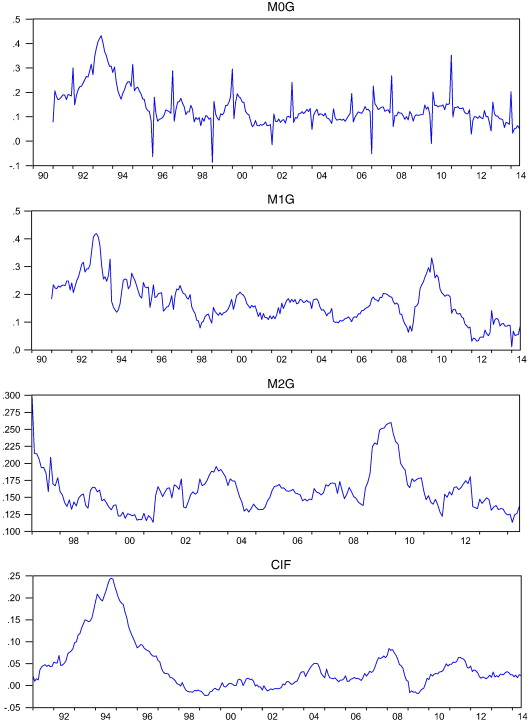
\includegraphics[]{image/1.jpg}
    \caption{ Time-series plots of money growth and inflation in China. $M_0$G, $M_1$G, and $M_2$G represent the growth rates of $M_0$, $M_1$, and $M_2$, respectively, while CIF represents the inflation rates.}
\end{figure}

\begin{table}
    \caption{Descriptive Statistics of money growth and inflation within each cycle.}\label{tbl1}
	\begin{tabular*}{\tblwidth}{@{}LLLLLLLLL@{}}
	    \toprule
	    Variable & Cycle & Period & Observations & Peak time & Maximum ($\%$) & Minimum ($\%$) & Mean ($\%$) & SD \\ % Table header row
	    \midrule
	    $M_0G$ & 1st & 1991.01–1994.06 & 42 & 1993.06 & 0.4323 & 0.0791 & 0.2558 & 0.0843 \\
		   & 2nd & 1994.07–1998.06 & 48 & 1995.01 & 0.3149 & -0.0630 & 0.1470 & 0.0661 \\
		   & 3rd & 1998.07–2002.01 & 43 & 2000.01 & 0.2962 & -0.0870 & 0.1060 & 0.0599 \\
		   & 4th & 2002.02–2005.01 & 36 & 2003.01 & 0.2415 & 0.0484 & 0.1045 & 0.0302 \\
		   & 5th &2005.02–2008.11 & 46 & 2008.01 & 0.2678 & -0.0518 & 0.1156 & 0.0443 \\
		   & 6th & 2008.12–2011.12 & 37 & 2011.01 & 0.3522 & -0.0101 & 0.1320 & 0.0488 \\
		   & 7th & 2012.01–2014.06 & 30 & 2014.01 & 0.2022 & 0.0287 & 0.0875 & 0.0355 \\
	    $M_1G$ & 1st & 1991.01–1994.04 & 40 & 1993.04 & 0.4185 & 0.1357 & 0.2662 & 0.0714 \\
		   & 2nd & 1994.05–1998.06 & 50 & 1995.01 & 0.2764 & 0.0793 & 0.1942 & 0.0434 \\
		   & 3rd & 1998.07–2002.01 & 43 & 2000.06 & 0.2080 & 0.0967 & 0.1434 & 0.0300 \\
		   & 4th & 2002.02–2004.12 & 35 & 2002.11 & 0.1845 & 0.1124 & 0.1599 & 0.0216 \\
		   & 5th & 2005.01–2008.11 & 47 & 2007.08 & 0.2034 & 0.0637 & 0.1423 & 0.0379 \\
		   & 6th & 2008.12–2011.12 & 37 & 2010.01 & 0.3315 & 0.0678 & 0.1832 & 0.0735 \\
		   & 7th & 2012.01–2014.06 & 30 & 2013.01 & 0.1418 & 0.0115 & 0.0692 & 0.0298 \\
	    $M_2G$ & 1st &/&/&/&/&/&/&/ \\
		   & 2nd & 1997.01–1998.06 & 18 & 1997.01 & 0.2975 & 0.1325 & 0.1810 & 0.0396 \\
		   & 3rd & 1998.07–2001.05 & 35 & 1999.04 & 0.1649 & 0.1134 & 0.1354 & 0.0155 \\
		   & 4th & 2001.06–2004.08 & 39 & 2003.08 & 0.1953 & 0.1297 & 0.1652 & 0.0162 \\
		   & 5th & 2004.09–2008.11 & 51 & 2008.01 & 0.1733 & 0.1285 & 0.1529 & 0.0123 \\
		   & 6th & 2008.12–2011.09 & 34 & 2009.11 & 0.2600 & 0.1222 & 0.1916 & 0.0427 \\
		   & 7th & 2011.10–2014.06 & 33 & 2012.09 & 0.1805 & 0.1134 & 0.1550 & 0.0170 \\
	    $CIF$ & 1st & 1991.01–1998.12 & 96 & 1994.10 & 0.2445 & -0.0151 & 0.0880 & 0.0737 \\
		& 2nd & 1999.01–2002.04 & 40 & 2001.05 & 0.0169 & -0.0222 & -0.0018 & 0.0110 \\
		& 3rd & 2002.05–2006.03 & 47 & 2004.08 & 0.0507 & -0.0103 & 0.0166 & 0.0171 \\
		& 4th & 2006.04–2008.12 & 33 & 2008.02 & 0.0844 & 0.0118 & 0.0427 & 0.0239 \\
		& 5th & 2009.01–2012.07 & 43 & 2011.07 & 0.0647 & -0.0181 & 0.0267 & 0.0253 \\
		& 6th & 2012.08–2014.06 & 23 & 2013.10 & 0.0318 & 0.0158 & 0.0232 & 0.0045 \\
	    \bottomrule
	\end{tabular*} 
\end{table}

Taking advantage of wavelet tools, the rectified wavelet power spectrums of money growth and inflation series are also estimated in \hyperref[fig:2]{Fig. 2}. 
\footnote{We thank Eric K. W. Ng for providing us with the modified package that has the bias problem rectified. The bias problem is presented by \cite*{liu2007} and \cite*{veleda2012}. They point out that the conventional wavelet power spectrum are simply defined as the square of the modulus of wavelet transform (i.e., the CWT in this paper), which will induce the biased or distorted wavelet power where the low-frequency (high-scale) oscillations tend to be overestimated. Using the proposed normalizing factor $s^{-1}$ (i.e., with the standard wavelet power spectrum divided by the wavelet scale parameter), they have the biased wavelet power simply rectified. Note that, however, the similar problem does not occur in estimation of wavelet coherency in this paper since the normalizing factor $s^{-1}$ has already been included in formula (6). In other words, the rectified auto- and cross-wavelet power spectrum are used instead in formula (6), therefore no further rectification is needed for the wavelet coherency in the present paper.}
The thick black contours designate the $5\%$ significance level estimated from Monte Carlo simulations using a phase randomized surrogate series. The regions below the thin black lines are the cone of influence (COI) in which edge effects cannot be ignored.
\footnote{Following \cite*{torrence1998} and \cite{grinsted2004}, when transforming finite-length time series into wavelets, errors probably occur at both the ends of wavelet power spectrum and wavelet coherency, as the CWT assumes that the series are cyclical. The method to avoid the errors is to pad the ends of the series with zeros. However, zero padding will cause discontinuities at the end points, especially as one moves to larger scales (lower frequencies) and declines in the amplitude (variance) near the edges as more zeroes enter the transform. As a consequence, due to this type of edge effect, we cannot distinguish inside the COI whether the decline in lower frequencies is a true decline or an artifact of the zero padding. Therefore, it must take special attention not to misread the results in the COI.}
We can see that $M_0$ growth shows intensive volatilities at shorter time scales (i.e., higher frequencies) in accordance with the highest liquidity of $M_0$ in comparison to $M_1$ and $M_2$. By contrast, $M_1$ and $M_2$ growth share similar wavelet power during the 1992–1998 and 2008–2011 periods, corresponding to the first, second, and sixth cycles of them as mentioned above. Moreover, the result that $M_1$ and $M_2$ growth mainly varies across 2-4 years' time scales is much the same with the cycle lengths indicated by \hyperref[tbl1]{Table 1}. As for inflation series, higher wavelet power mainly exists in two periods, 1992–1998 and 2007–2011, corresponding to the higher volatilities during its first, fourth, and fifth cycles. Particularly, the result that inflation varies across 1- to 8-year time scales during 1992–1998 is also greatly in line with the 96-month cycle for this period in \hyperref[tbl1]{Table 1}.

\begin{figure}[h]\label{fig:2}
    \centering
    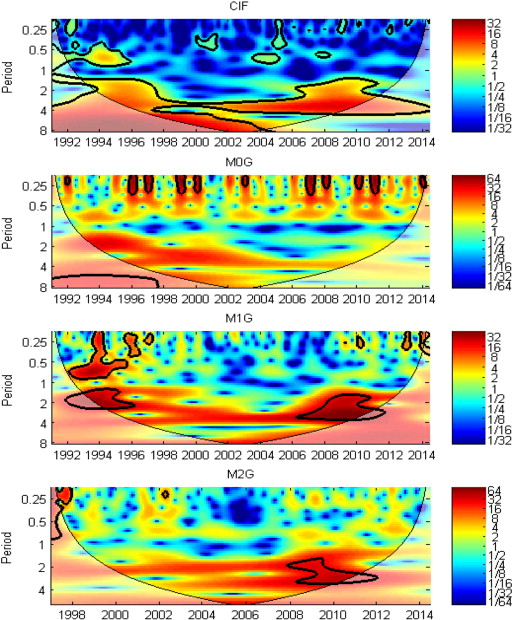
\includegraphics[]{image/2.jpg}
    \caption{The squared wavelet coherency and phase difference between $M_2$G and C$_I$F from 1997 to 2013. M2G represents M2 growth rates, while CIF represents the inflation rates. The x-axis refers to time periods. The y-axis to scales or frequencies (measured in years). The color corresponds to the strength of the correlation.}
\end{figure}

It may seem that almost the same results are presented in \hyperref[tbl1]{Table 1} and \hyperref[fig:2]{Fig. 2}. However, using wavelet-based spectral tools, \hyperref[fig:2]{Fig. 2} provides significant evidence in a time-frequency space where structural changes of money growth and inflation can be read off in a highly visual way. Specifically, the very high volatility of money growth in the first cycle is probably the consequence of the famous talk delivered on Xiao-ping Deng's south tour in 1992, which greatly stimulated China's money growth in 1992–1993 followed by a sharp decline in 1994 due to an ever-increasing inflation. In the second cycle, the PBoC begins to make mild but frequent adjustments in money growth, ensuring that China successfully cushioned the economic fallout at the end of 1996. As a result, the volatilities of $M_0$ and $M_1$ growth become milder within this cycle. The relatively high volatility in the sixth cycle can be attributed to the global financial crisis of 2008–2009. Under crisis circumstances, an unprecedented expansionary monetary policy is conducted by the PBoC to arrest the economic downturn. Consequently, money growth hits a record high in late 2009. However, after 2010, it starts to fall rapidly due to an overheating economy. According to the estimated wavelet power of inflation in \hyperref[fig:2]{Fig. 2}, we find that the wavelet power varies across longer time scales (i.e., lower frequencies) in the 1999–2007 period, which may be indicative of high inflation persistence in a low-inflation environment. However, despite its utility, the wavelet power spectrum cannot reveal any local correlation and lead-lag relationship between time series. Therefore, wavelet coherency and phase-difference tools are proposed in the empirical section to reveal the time- and frequency-varying relationship between money growth and inflation for China.

\section{Empirical results}\label{sec:5}
In this section, we plot wavelet coherencies and phase differences between money growth and inflation for China in \hyperref[fig:3]{Figs. 3–5}.
\footnote{We thank Alask Grinsted for providing us with the wavelet package to estimate the wavelet coherency and phase difference between money growth and inflation in China.}
    As mentioned before, the results inside the COI and the regions above the $5\%$ significance level are not reliable indications of correlations and lead-lag suggestion.We classify the frequency on the y-axis into three bands: ~1-year time scale, 1- to 4-year time scales, and 4- to 8-year time scales, corresponding to short-run, medium-run, and long-run relationships between money growth and inflation. For a better comparison, the relationship of the growth rates of $M_0$, $M_1$, and $M_2$ relative to inflation is analyzed as follows.

\begin{figure}[h]\label{fig:3}
    \centering
    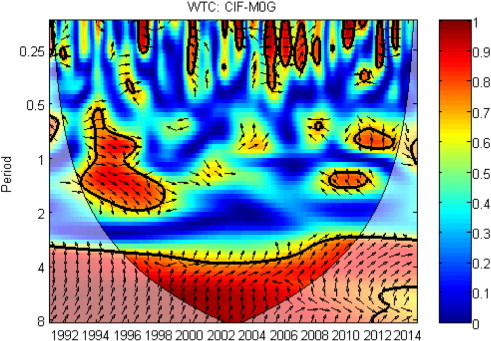
\includegraphics[]{image/3.jpg}
    \caption{The squared wavelet coherency and phase difference between $M_0G$ and CIF from 1991 to 2013. $M_0G$ represents $M_0$  growth, while CIF represents the inflation rates. The x-axis refers to time periods. The y-axis is scales (measured in years). The color corresponds to the strength of the correlation.}
\end{figure}

\subsection{The relationship between \boldmath $M_0$ growth and inflation}
In the ~1-year time scale, high and intensive correlations between $M_0$ growth and inflation can be observed in \hyperref[fig:3]{Fig. 3}. In 1994–1996, $M_0$ growth has a positive and strong impact on inflation with a coefficient of wavelet coherency close to $0.8$. However, it starts to negatively impact inflation in 1996–1997 and 2000–2001, which fits the fact that an obvious increase in $M_0$ growth does not head off a continuous decline in inflation during these years. Until the 2004–2008 period, the positive relationship reoccurs between $M_0$ growth and inflation, followed by a negative impact of $M_0$ growth on inflation in the first half of 2012 as well. It seems unusual that $M_0$ growth negatively impacts inflation in the short run for several years, which greatly conflicts with \cite{xie2004}, \cite{roffia2007}, \cite{Zhang2012}, \cite{Yu2012} but accords well with \cite{shuai2002} and \cite{wu2002}. However, more unusually, $M_0$ growth and inflation alternates between positive and negative relationships over time in China. The same results can also be observed for the 1- to 4-year time scales (1- to 2-year time scales in particular). $M_0$ growth has a strong and positive effect on inflation in 1993– 1999, while it turns to negatively impact inflation in 2009–2010 in 1- to 4-year time scales.

\begin{figure}[h]\label{fig:4}
    \centering
    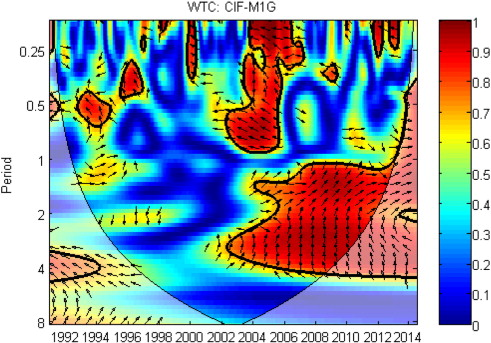
\includegraphics[]{image/4.jpg}
    \caption{The squared wavelet coherency and phase difference between $M1G$ and CIF from 1991 to 2013. $M_1G$ represents $M_1$ growth while CIF represents the inflation rates. The x-axis refers to time periods. The y-axis to scales (measured in years). The color corresponds to the strength of the correlation.}
\end{figure}

\begin{figure}[h]\label{fig:5}
    \centering
    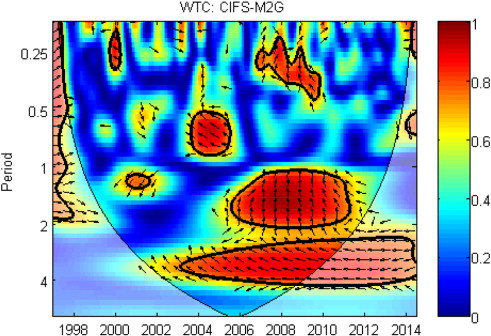
\includegraphics[]{image/5.jpg}
    \caption{The squared wavelet coherency and phase difference between $M_2G$ and $CIF$ from 1997 to 2013. $M_2G$ represents $M_2$ growth rates, while $CIF$ represents the inflation rates. The x-axis refers to time periods. The y-axis to scales or frequencies (measured in years). The color corresponds to the strength of the correlation.}
\end{figure}

The phase differences represented as arrows may provide us with reasonable clues to explain these unusual findings. In the -1-year time scale, arrows pointing to the right and downwards in 1994–1996 and pointing to the left and upwards in 1996–1997, 2000–2001, and 2012 indicate that inflation lags behind $M_0$ growth by 1-2 months in the short run. In the 1- to 4-year time scales, the same arrow directions in 1993–1999 and 2009–2010 also indicate that inflation lags behind $M_0$ growth by 4-6 months in the medium run. That is, the significant lag effects of $M_0$ growth on inflation should be responsible for the unusual relationships in the short and medium run. In fact, the lag effects of money growth on inflation are often proved to be unavoidable facts, especially in monthly analysis (\citealp{friedman1956}; \citealp{meiselman1969}; \citealp{Zhang2008}; \citealp{zhang2009}).

The correlation between $M_0$ growth and inflation is more stable at low frequencies relative to high frequencies. In the 4- to 8-year time scales, a high and positive impact of $M_0$ growth on inflation can be found during 1996–2009.11 In addition, a coefficient of wavelet coherency close to 1 means that $M_0$ growth and inflation are related one-for-one in the long run, which is consistent with \cite*{MacCandless1995} and \cite{Grauwe2005}, as well as the modern QTM in particular. Additionally, the phase difference provides evidence once again that inflation significantly lags behind $M_0$ growth in the long run, with a time lag of 3–6 years, which is longer than 1–1.5 years claimed by \cite{friedman1956} and even longer than 4 years, as argued by \cite*{liukopin2002}.

\subsection{The relationship between \boldmath $M_1$ growth and inflation}
$M_1$ growth and inflation are more linked at 1- to 4-year time scales, as shown in \hyperref[fig:4]{Fig. 4}; thus, we focus on the results at the shorter time scales. At the $\sim$1-year time scale, we find that $M_1$ growth has a high and negative effect on inflation in 1993–1995, 1996–1997, 2000–2001, and 2003–2007, with an average coefficient of wavelet coherency close to $0.8$. This strongly supports the argument by \cite{shuai2002} and \cite{wu2002}. However, unlike Shuai (2002) and Wu (2002), who claim that the negative link is stable over the 1993–2001 period without distinguishing between short-run and long-run links, this paper shows that the negative link is much less stable in the short run. In addition, the negative link can also be found in this paper for the recent period of 2003–2007. That is, such an unusually negative link between $M_1$ growth and inflation is more common for China in the short run, which would inevitably weaken the effectiveness of monetary policy in managing inflation. With regard to the reason for the short-run negative link, it can be revealed well by the phase differences, which indicate that $M_1$ growth has a significant lag effect on inflation in the short run.

In the 1- to 4-year time scale, $M_1$ growth turns to positively impact inflation in 2002–2011, which is entirely different from the short-run negative relationship. In this sense, it is confirmed that the negative relationship between $M_1$ growth and inflation is only found in the short run. By contrast, in the medium run, the positive relationship coupled with a coefficient of wavelet coherency close to $1$ indicates that $M_1$ growth relates to inflation one-for-one. This means that the medium-run relationship between $M_1$ growth and inflation supports the modern QTM as well after the early 2000s. It can be interpreted that $M_1$ growth plays a more effective role in managing inflation in the medium run. Meanwhile, it can also be inferred from a time-domain view that China's monetary policy has gained improvements in controlling inflation since the early 2000s. However, it should not be ignored that inflation lags behind $M_1$ growth with a time lag of 1.5–2 years in the medium run. That is, in general, the lag effects of $M_1$ growth on inflation in the short and medium run should be largely responsible for the short-run negative relationship, and only when the lag effect has been weakened can the effectiveness of monetary policy in managing inflation be further enhanced in China.

\subsection{The relationship between \boldmath $M_2$ growth and inflation}
As shown in \hyperref[fig:5]{Fig. 5}, in the $\sim$1-year time scale, $M_2$ growth has a strong and negative effect on inflation in 2000–2001 and 2003–2005. As discussed above, the same link has already been found between $M_1$ growth and inflation in these years. Therefore, it can be concluded that the negative link during these years does not occur by chance. Except for the lag effect of money growth and inflation, high inflation persistence in a low-inflation environment also contributes to the negative link during these years, when China's economy experiences a notably low rate of inflation. Until the 2007–2010 period, inflation in turn has a large and positive impact on $M_2$ growth, with phase differences indicating that $M_2$ growth lags behind inflation by 1–2 months in the short run. This finding is totally different from the result in previous years, probably as a result of the external demand shock caused by the global financial crisis. Especially in late 2008, when the crisis breaks out, China's inflation drops sharply from $8\%$ to below $0\%$ in several months, swiftly followed by a spike of $M_2$ growth in early 2009. In this sense, our finding shows that China's money policy has responded in a timely manner to the sharp decline in inflation during the global financial crisis.

Different results can be observed across longer time scales. First, in the 1- to 2-year time scales, $M_2$ growth positively impacts inflation in 2005–2011 with a value of wavelet coherency close to $1$, very similar to the results for $M_0$ growth and inflation in the long run and $M_1$ growth and inflation in the medium run. The result implies that the relationship between $M_2$ growth and inflation in the medium run supports the modern QTM as well. However, it is noted that China's inflation would eventually respond one-for-one to $M_2$ growth with a time lag of 9–18 months, indicating a much weaker lag effect of $M_2$ growth on inflation than that of $M_1$ growth on inflation. Second, in the 2- to 4-year time scales, a negative effect of $M_2$ growth on inflation can be found very stably in the 2002–2010 period.
\footnote{2 Considering the edge effects inside the COI, we only focus on the long-term relationship between $M_2$ growth and inflation during the 2002-2010 period.}
This finding presents an explanation for why so much money has not brought high inflation to China in recent years, and it is also an indication for China that inflation will be maintained at a low level at least in the next 2 years. Our result strongly support \cite{Yanyan2009}, who point out that money growth drives inflation moving in a hump shape and even brings deflation in the medium or long run, namely, the so-called deflation effect of expansionary monetary policy in China.

Lastly, similar to $M_1$ growth and inflation, no correlation with high coherency can be found between $M_2$ growth and inflation in the 4- to 8-year time scales. This indicates that there are no long-run relationships between $M_1$ and inflation as well as $M_2$ growth and inflation, which is greatly inconsistent with the result that inflation lags behind $M_0$ growth by 3–6 years in the long run. In this sense, we can therefore conclude that $M_1$ and $M_2$ growth has a much weaker lag effect on inflation than that of $M_0$ growth on inflation. Based on the above results, we in fact plot a three-dimensional picture for the relationship between money growth and inflation in China. First, from a time-domain view, we find strong but not homogenous links in the mid-1990s and the period since the early 2000s. Especially since the early 2000s, money growth has shown a much stronger effect on inflation, which provides significant evidence that China's monetary policy has started to perform well in serving as a tool to manage inflation. Second, from a frequencydomain view, we conclude in general that the short-run relationship between money growth and inflation is much less stable over time than the relationship in the medium and long run. In other words, the short-run relationship tends to deviate from the wellestablished positive link between money growth and inflation because it is more sensitive to internal or external temporary shocks. 

As a result, money growth negatively impacts inflation in the short run, but it turns to positively impact inflation in the medium or long run. Therefore, it can be concluded for China that the long-run relationship between $M_0$ growth and inflation supports the modern QTM, while the medium-run relationship between $M_1$ and $M_2$ growth relative to inflation supports the modern QTM. Third, to make a further comparison among $M_0$, $M_1$, and $M_2$, we find that inflation is more linked with $M_0$ growth in the short and long run, but it is more linked with $M_1$ and $M_2$ in the medium run. In addition, $M_0$ growth has the most significant lag effect on inflation, while $M_2$ growth has the weakest lag effects on inflation. The lag effect of $M_1$ growth on inflation is found between the two. Therefore, we suggest that the severe lag effect of money growth on inflation should be responsible largely for the unusually negative relationship in the short or medium run. Moreover, it has inevitably weakened the effectiveness of monetary policy in inflation management in China.

In this paper, wavelet analysis provides an additional insight into the dynamic relationship between money growth and inflation in China. Although the relationship in China is not stable over time and even exhibits short-run deviations from the positive link, it actually fits well the fact that China has experienced economic transitions and structural changes in monetary policy over the past two decades. In 1994, a profound transition to a socialist market economy system has largely reduced price controls. After that point, prices start to be more freely determined by the interaction between supply and demand. In 1995, inflation management has formally become the primary target of the PBoC, and the money supply and hence money growth then began to serve as the intermediate targets of monetary policy after 1 year. In 1997, the shortage economy that had existed in China for a very long time disappeared after the Asian financial crisis, implying that the level of inflation has become lower than before in general. Since 2001, the macro-control once dominated by fiscal policy in China has been changed, and hence, the role of monetary policy in economy has been strengthened. At the same time, the PBoC also has started to issue a quarterly report of the implementation of monetary policy, which helps to enhance policy transparency and manage inflation expectations. Since 2002, ever-increasing foreign exchange reserves after entering into the WTO have accelerated money growth and brought potential pressure to inflation for China. In recent years, the global financial crisis also brings a huge shock to the relationship between money growth and inflation. All of these internal and external events could bring temporary shocks or induce structural changes to the relationship between money growth and inflation in China. Therefore, we should not simply argue a positive or negative relationship between them; rather, we should consider specific economic backgrounds and utilize more scientific methods and thus gain an accurate look into the complicated relationship for China.

Our results have important implications for policymaking in China. Primarily, the key to improving the effectiveness of monetary policy operations is to reduce the significant lag effects of money growth on inflation. In short, only when the lag effect has been weakened can the effectiveness of monetary policy on managing inflation be further enhanced in China. For this purpose, China needs to deepen its market-oriented reform and enhance the transparency of monetary policy, thus helping anchor inflation expectations and better maintain price stability for the future. In addition, it is noted that a deflation effect of money growth on inflation in the medium run, possibly as a result of people's expectations, presents an indication for China that inflation would be maintained at a low level in the next 2 years. This implies that at least in the next 2 years, there is no need to be concerned with the potential inflation pressure as mentioned at the beginning of this paper. Another noteworthy implication is that volatile money growth is always followed by volatile inflation, as shown by the facts during the mid-1990s and the end-2000s. Therefore, it is critical to keep a reasonable and steady money growth in China for long-run inflation stability.

\section{Conclusions}\label{sec:6} 
Wavelet analysis provides new evidence of the time-frequency relations between money growth and inflation in China. From a time-domain view, we find strong but not homogenous links between money growth and inflation in the mid-1990s and the period since the early 2000s. Particularly since the early 2000s, China's monetary policy has been proved to perform well as a tool to manage inflation. From a frequency-domain view, our findings show that money growth and inflation are positively and stably related one-to one in the medium or long run while they deviates from the positive relation in the short run due to temporary shocks and a significant lag effect of money growth on inflation. Moreover, we can also conclude that the long-run relationship between $M_0$ growth and inflation supports the modern QTM, while the medium-run relationship between $M_1$ growth and inflation as well as $M_2$ growth and inflation supports the modern QTM. In general, however, our results fit well with the fact that China has experienced economic transitions and structural adjustments in monetary policy over the past two decades. Therefore, it is essential to consider specific economic backgrounds and utilize more scientific methods, can thus have an accurate look into such a complicated relationship for China.


% To print the credit authorship contribution details
\printcredits

%% Loading bibliography style file
%\bibliographystyle{model1-num-names}
\bibliographystyle{cas-model2-names}

% Loading bibliography database
\bibliography{cas-refs}

% Biography
\bio{}

\end{document}

